\documentclass[12pt,a4paper]{article}

% 使用中文宏包
\usepackage[UTF8]{ctex}
\usepackage{graphicx} %插入图片的宏包
\usepackage{float} %设置图片浮动位置的宏包
\usepackage{enumerate}
\usepackage[strings]{underscore}
\usepackage{times}
\usepackage{epsfig}
\usepackage{amsmath}
\usepackage{amssymb}
\usepackage{overpic}
\usepackage{listings}
\usepackage{color}
\usepackage{enumitem}
\setenumerate[1]{itemsep=0pt,partopsep=0pt,parsep=\parskip,topsep=5pt}
\setitemize[1]{itemsep=0pt,partopsep=0pt,parsep=\parskip,topsep=5pt}
\setdescription{itemsep=0pt,partopsep=0pt,parsep=\parskip,topsep=5pt}

\definecolor{mygreen}{rgb}{0,0.6,0}
\definecolor{mygray}{rgb}{0.5,0.5,0.5}
\definecolor{mymauve}{rgb}{0.58,0,0.82}
\lstset{ %
  backgroundcolor=\color{white},   % choose the background color
  basicstyle=\footnotesize,        % size of fonts used for the code
  breaklines=true,                 % automatic line breaking only at whitespace
  captionpos=b,                    % sets the caption-position to bottom
  commentstyle=\color{mygreen},    % comment style
  escapeinside={\%*}{*)},          % if you want to add LaTeX within your code
  keywordstyle=\color{blue},       % keyword style
  stringstyle=\color{mymauve},     % string literal style
}

\usepackage[pagebackref=true,breaklinks=true,letterpaper=true,colorlinks,bookmarks=false]{hyperref}


\def\httilde{\mbox{\tt\raisebox{-.5ex}{\symbol{126}}}}


\graphicspath{{figures/}}

\setcounter{page}{1}

\begin{document}


%%%%%%%%% TITLE

\title{论文阅读笔记:差分隐私}
\author{纳文琪}
\maketitle


\section{差分隐私保护及其应用\cite{熊平2014}}
\subsection{引言}
\paragraph{基于分组的隐私模型} “k-anonymity及其扩展模型被称为基于分组的隐私模型”,这些模型主要存在两个主要的缺陷:
\begin{itemize}
	\item “并不能提供足够的安全保障,他们总是因新型攻击的出现而需要不断完善”。“出现这一局面的原因在于,基于分组的隐私保护模型的安全性与攻击者所掌握的背景知识相关,而所有可能的背景知识很难被充分定义。”
	\item “这些早期的隐私保护模型无法提供一种有效且严格的方法来证明其隐私保护水平,因此当模型参数改变时,无法对隐私保护水平进行定量分析。”
\end{itemize}
差分隐私能够解决传统隐私保护模型的两个缺陷。
\subsection{差分隐私保护模型}
\paragraph{基本思想} “设对数据集D进行任意操作f,得到f(D),如果将A从D中删除后,得到的结果仍然为f(D),则可以认为A的信息并没有因为包含在D中而产生额外的风险。”

\subsubsection{基本概念}
\paragraph{隐私保护机制} “对D的各类映射函数被定义为查询,用$F=\left \{ f_1, f_2,... \right \}$表示一组查询,算法M对查询F的结果进行处理,使之满足隐私保护的条件,此过程称为隐私保护机制。”
\paragraph{邻接数据集} “属性结构相同的数据集D和D',两者的对称差记为$D\Delta D'$,若$|D\Delta D'|=1$,则称D和D'为邻接数据集。”
\paragraph{差分隐私} 设$P_M$是算法M所有可能的输出构成的集合,$S_M$是$P_M$子集,若算法满足:
\begin{equation}
	Pr[M(D)\in S_M] \leq e^\varepsilon \times Pr[M(D')\in S_M]
\end{equation}
则称算法M提供$\varepsilon$-差分隐私保护。
\paragraph{隐私保护预算} 上式中的$\varepsilon$称为隐私保护预算,用来控制算法M在D和D'上获得相同输出的概率比值,它通常取比较小的值。$\varepsilon$越小,表示隐私保护水平越高,当$\varepsilon$为0时,保护水平最高。
\paragraph{敏感度} “差分隐私保护可以通过在f的返回值中加入噪声来实现。敏感度是决定加入噪声量大小的关键参数。”
\paragraph{全局敏感度} 设函数$f:D\rightarrow R^d$,对于邻近数据集D和D',函数f的全局敏感度定义为:
\begin{equation}
	GS_f=\max_{D,D'} \left \| f(D)-f(D') \right \|_1
\end{equation}
“函数的全局敏感度由函数本身决定。当GS较大时,必须在函数输出中添加足够大的噪声才能保证隐私安全,导致数据可用性较差。”
\paragraph{局部敏感度} 设函数$f:D\rightarrow R^d$,对于邻近数据集D和D',函数f在D上的局部敏感度定义为:
\begin{equation}
	LS_f(D) = \max_{D'} \left \| f(D)-f(D') \right \|_1
\end{equation}
“局部敏感度由函数f及给定数据集D共同决定。”GS和LS之间的关系可以表示为:
\begin{equation}
	GS_f=\max_D(LS_f(D))
\end{equation}
\paragraph{平滑上界} “LS在一定程度上体现了数据集的数据分布特征,直接应用会泄露数据集中的敏感信息。因此,LS的平滑上界被用来与LS一起确定噪声量的大小。”对于$\beta>0$,若函数$S:D\rightarrow R$满足$S(D) \geq LS_f(D)$且$S(D) \leq e^\beta \times S(D')$,则称S是f的LS的$\beta$-平滑上界。
\paragraph{平滑敏感度} 函数f的$\beta$-平滑敏感度定义为:
\begin{equation}
	S_{f,\beta}(D)=\max_{D'}(LS_f(D')\times e^{-\beta |D\Delta D'|}
\end{equation}
\subsubsection{差分隐私保护算法的组合性质}
\paragraph{} “一个复杂的隐私保护问题,通常需要多次应用差分隐私保护算法,为了保证整个过程的隐私保护水平控制在给定的预算之内,需要合理地将全部预算分配到整个算法的各个步骤中。”
\paragraph{序列组合性} “设有算法$M_1,...,M_n$,其预算分别是$\varepsilon_1,...,\varepsilon_n$,那么对同一个数据集D,由这些算法构成的组合算法$M(M_1(D),...,M_n(D))$提供$\sum_{i=1}^n \varepsilon_i$-差分隐私保护。”也就是说,“一个差分隐私保护算法序列构成的组合算法,其提供的隐私保护水平为全部预算的总和”。
\paragraph{并行组合性} “设有算法$M_1,...,M_n$,其预算分别是$\varepsilon_1,...,\varepsilon_n$,那么对于不相交的数据集$D_1,...,D_n$,由这些算法构成的组合算法$M(M_1(D_1),...,M_n(D_n))$提供$(\max \varepsilon_i)$-差分隐私保护”。此时算法系序列构成的组合算法提供的隐私保护水平取决于算法序列中的保护水平最差者。
\subsubsection{实现机制}
\paragraph{} 根据差分隐私保护的要求,不同的问题有不同的实现方法,即机制。最基础的两种机制是Laplace机制和指数机制。
\paragraph{Laplace分布} 两个指数型随机变量之差满足Laplace分布。其概率密度为:
\begin{equation}
	f(x|\mu,b) = \frac{1}{2b}e^{-\frac{|x-\mu|}{b} }
\end{equation}
其图像呈尖沙堆状,如图\ref{laplace-distribution} 所示。
\begin{figure}[H]
	\centering
	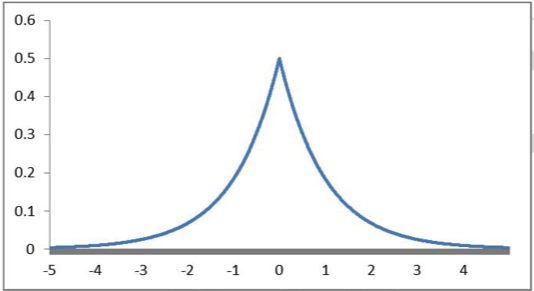
\includegraphics[width=0.6\textwidth]{../images/laplace-distribution.png}
	\caption{Laplace分布概率密度函数}
	\label{laplace-distribution}
\end{figure}

\paragraph{Laplace机制} Laplace机制仅适用于数值型结果的保护,通过向查询结果中加入服从Laplace分布的随机噪声来实现差分隐私保护。令设数据集D,函数f的敏感度为$\Delta f$,那么随机算法$M(D)=f(D)+Y$提供$\varepsilon$-差分隐私保护,其中$Y \sim Lap(\frac{\Delta f}{\varepsilon})$为随机噪声,服从尺度为$\frac{\Delta f}{\varepsilon}$的Laplace分布。

\paragraph{指数机制} 适用于非数值型查询结果。设随机算法M,输出为一实体对象$r \in Range$,函数$q(D,r)\rightarrow R $为可用性函数,$\Delta q$为函数$q(D,r)$的敏感度。若算法M以正比于$e^{\frac{\varepsilon q(D,r)}{2\Delta q}}$的概率从Range中选择并输出r,那么算法M提供$\varepsilon$-差分隐私保护。

\subsection{基于隐私保护的数据发布(PPDR)}
\paragraph{} PPDR研究的问题是如何在满足差分隐私的条件下保证发布数据或查询结果的精确性。根据实现环境可分为交互式数据发布和非交互式数据发布两种。
\subsubsection{交互式数据发布}
\paragraph{} “在交互式环境下,用户向数据管理者提出查询请求,数据管理者根据查询请求对数据集进行操作并将结果进行必要的干扰后反馈给用户,用户不能看到数据集全貌,从而保护数据集中的个体隐私”。具体可描述为:“给定数据集D和查询集合F,需寻求一种数据发布机制,使其能够在满足差分隐私保护的条件下逐个回答F中的查询,直到耗尽全部隐私保护预算”。“对于F中的任意f,设定一个足够小的实数$\delta$,查询结果精度$\alpha$应满足:
\begin{equation}
	Pr_{f\in F}[|f(D)-M(f(D))|\leq \alpha]\geq 1-\delta
\end{equation}
其中$f(D)$是查询结果,$M(f(D))$是对M的干扰结果。”
\subsubsection{非交互式数据发布} “在非交互式环境下,数据管理者针对所有可能的查询,在满足差分隐私的条件下一次性发布所有查询的结果。或者,数据管理者发布一个原始数据集的“净化”版本,这是一个不精确的数据集,用户可对该版本的数据集自行进行所需的查询操作”。可表述为:“给定D和F,需寻求一个数据发布机制,使其能够在满足差分隐私保护的条件下一次性回答F中所有的查询”。

\section{本地化差分隐私研究综述\cite{2018本地化差分隐私研究综述}}
\subsection{引言}
\paragraph{} "传统的差分隐私技术将原始数据集中到一个数据中心,然后发布满足差分隐私的相关统计信息,我们称之为中心化差分隐私(Centralized Differential Privacy)技术.因此,中心化差分隐私对于敏感信息的保护始终基于 一个前提假设:可信的第三方数据收集者,在不可信第三方数据收集者的场景下,本地化差分隐私(Local Differential Privacy)技术应运而生"
\paragraph{} "本地化差分隐私技术继承自中心化差分隐私技术,同时扩展出了新的特性,使该技术具备两大特点:1)充分 考虑任意攻击者的背景知识,并对隐私保护程度进行量化;2)本地化扰动数据,抵御来自不可信第三方数据收集 者的隐私攻击."
\paragraph{} "对本地化差分隐私的研究和应用,主要考虑以 下两个方面问题:(1)如何设计满足 -本地化差分隐私的数据扰动算法,以保护其中的敏感信息;(2)数据收集者 如何对查询结果进行求精处理,以提高统计结果的可用性."
\paragraph{研究方向} "本地化差分隐私技术的研究方向包括扰动机制的研究以及统计数据的发布.本地化差分隐私的扰动机制主要包括随机响应、信息压缩和扭曲两种."本地化差分隐私的统计数据发布包括:单值频数发布、多值频数发布和均值发布。
\subsection{基于本地化差分隐私的数据保护框架}
\paragraph{} "交互式和非交互式数据保护框架的最大区别在于输出结果之间的关联性.1)交互式框架适用于 最终输出结果与前 i 个输出有依赖关系的情形.2)非交互式框架适用于前后的输入输出之间无依赖关系的情形."
\subsection{基于本地化差分隐私的单值频数统计}
\paragraph{} "单值频数统计是指每个用户只发送一个变量取值的情形,用户将数据发送给数据收集者后,数据收集者根 据已有的或统计得到候选值列表,统计其中每一个候选值的频数并进行发布."
\paragraph{RAPPOR方法} 变量以字符串表示,先将变量通过Bloom Filter表示成长度为h的向量,然后对向量进行一次随机扰动,得到PRR,再进行第二次随机扰动得到IRR,然后将扰动结果发送给数据收集者。"RAPPOR 方法的主要存在两个方面的缺陷:1)用户和数据收集者之间的传输代价比较高,即每个用户需要传输长度为 h 的向量给数据收集者;2)数据收集者需预先采集候选字符串列表,以进行频数统计."
\subsection{未来研究挑战} 
\paragraph{} "现有研究主要集中在两个方面:1)理论上,设计满足本地化差 分隐私的保护机制;2)方法上,对频数和均值两种统计结果进行保护."
\paragraph{复杂数据类型的本地化差分隐私保护} "目前,本地化差分隐私保护技术的研究主要还是针对简单的数据类型,然而,简单的数据类型对于当下空前的数据分析需求而言,还远远不够.以键值对数据(Key-value database)和图数据(Graph database)为例"
\paragraph{不同查询和分析任务的本地化差分隐私保护} "聚类分析是为了把性质相近的数据归入一类,典型应用如 客户群体发现、社区发现等;频繁模式挖掘的目的则是找出数据集中的频繁项集,进而发现模式规律,典型应用 如搜索日志分析、购买行为分析等.聚类分析和频繁模式挖掘都是数据分析中的常用方法,其中涉及的查询包 括计数查询、均值查询、范围查询和最值查询等.本地化差分隐私下,不仅要求能够支持不同的查询类型,还要 求扰动后的数据能够同时支持多种不同的查询.与中心化差分隐私不同,本地化差分隐私通过抵消添加在数据 中的正向和负向噪声来得到比较准确的统计结果,但就单条数据记录而言,通常扰动前后数据的偏差较大,这也 进一步加大了针对不同查询的难度."
\paragraph{基于本地化差分隐私的高维数据发布} "本地化差分隐私下的高维数据发布主要考虑三个方面的问题:1)如何在一定隐私预算 内衡量属性之间的关联性,从而进行降维处理;2)如何设计推理模型,最小化边缘分布到联合分布的近似误差,提 高数据可用性;3)如何控制高维数据在用户和数据收集者之间的通信代价."







\newpage
\section{Privacy-preserving deep learning\cite{shokri2015ppdl}}
\subsection{Introduction}
\paragraph{} 本文提出一种协调深度学习系统,用于权衡效用和隐私。系统运行多方使用自己的输入数据合作训练一个神经网络模型,而不需要共享。此技术的关键创新是,在训练期间选择性共享模型参数。参数共享运行多个参与者在没有显式的输入数据的共享的情况下,互相利用其它人的模型计算结果。

\subsection{相关工作}
\subsubsection{Privacy in ML}
\paragraph{} 当多方利用自有数据协同执行机器学习任务时,基于安全多方计算(secure multi-party computation, SMC)的技术帮忙我们计算的中间步骤的隐私。

\subsection{Distributed Selective SGD}
\paragraph{} 本文方法的核心是分布式的、协作的深度学习协议,它基于以下观察结果:
\begin{itemize}
	\item 梯度下降的过程中,对不同参数的更新本质上是独立的;
	\item 不同的训练数据集作用于不同的参数;
	\item 不同的特征对目标函数的作用并不相等。
\end{itemize}
\paragraph{} 在进行选择性SGD时,学习器选择一部分参数进行更新,可选择梯度较大的那部分参数。
\subsection{系统架构}
\paragraph{概述} 系统由一个管理全局参数的参数服务器和多个局部训练器(参与者)组成,他们之间通过参数选择协议交换参数。参数交换协议允许参与者独立地优化参数、避免过拟合。
\paragraph{Local training} 每个参与者都可以在本地训练神经网络的参数。假设本地维护$w^{(i)}$个参数。训练过程如下:
\begin{enumerate}
	\item 将$\theta_d \times |w^{(i)}|$个参数下载并更新到本地,并不下载更新全部参数;
	\item 运行一轮SGD;
	\item 计算$\Delta w^{(i)}$,即新旧参数之间的差值;
	\item 选择性地上传最多$\theta_u \times |w^{(i)}|$个参数到服务器。选择方法有:
	\begin{itemize}
		\item 最大值选择:选择最大的几个值进行上传;
		\item 带阈值的随机选择:从大于阈值$\tau$的值中随机选择上传;
	\end{itemize}
\end{enumerate}
另外,上传$\Delta w^{(i)}$的值之前,这些值将被截断在$[-\gamma, \gamma]$之间,以避免这些值泄露训练数据的太多信息。
\paragraph{为什么DSSGD能行?} 这主要是因为学习过程的随机性。在训练过程中随机更新局部参数会增加局部SGD的随机性。而由异步参数更新导致的随机性对于精确地训练神经网络非常有效。
\paragraph{Parameter exchange protocol} 交换协议有三种类型:
\begin{itemize}
	\item 轮询。每个参与者按固定顺序下载、训练并更新一部分参数,然后下一个参与者继续;
	\item 随机。所有参与者同时随机下载、训练并更新一部分参数,但参数的读取过程是加锁的,也就是具有原则性(atomic);
	\item 异步。同随机一样,但并不加锁。
\end{itemize}
\subsection{Evaluation}
\paragraph{数据集} 实验选用的数据集是MNIST和SVHN
\paragraph{神经网络架构} 分别采用MLP和CNN
\paragraph{实验设置} 
\paragraph{选择性SGD的实验结果} SSGD的实验得到了以下结论:
\begin{itemize}
	\item SSGD可以获得与SGD相同的精度;
	\item SGD和SSGD在总体上是类似的;
	\item SSGD甚至能够取得比SGD更高的精度,这是因为SSGD类似于给SGD加上了Dropout。
\end{itemize}
\paragraph{DSSGD的实验结果} 结果表明:
\begin{itemize}
	\item 任何形式的协作都可以获得比独立学习更高的精度;
	\item 参与者的数量比共享参数的比例对精度的影响更小。
\end{itemize}
\subsection{Privacy}
\subsubsection{防止直接泄露}
\paragraph{训练过程} 在此过程中,由于各自的数据都不共享,所以不存在泄露。
\paragraph{模型使用过程} 此过程中也不需要使用到训练数据,因此也不存在泄露。

\subsubsection{防止间接泄露}

\section{Deep learning with differential privacy\cite{abadi2016deep} }
\subsection{Introduction}
\paragraph{} 深度学习模型不应该暴露数据集中的隐私信息,出于这个考虑,本文提出了一种学习算法,以较小的隐私预算训练非凸、规模巨大的深度网络。
\subsection{Our Approach}
\subsubsection{差分隐私SGD算法}
\paragraph{} 保护SGD过程中的隐私,其实就是对梯度进行隐私保护。本文的方法是首先根据限界对梯度进行修剪,然后再加上噪声。算法如下。
\begin{figure}[H]
	\centering
	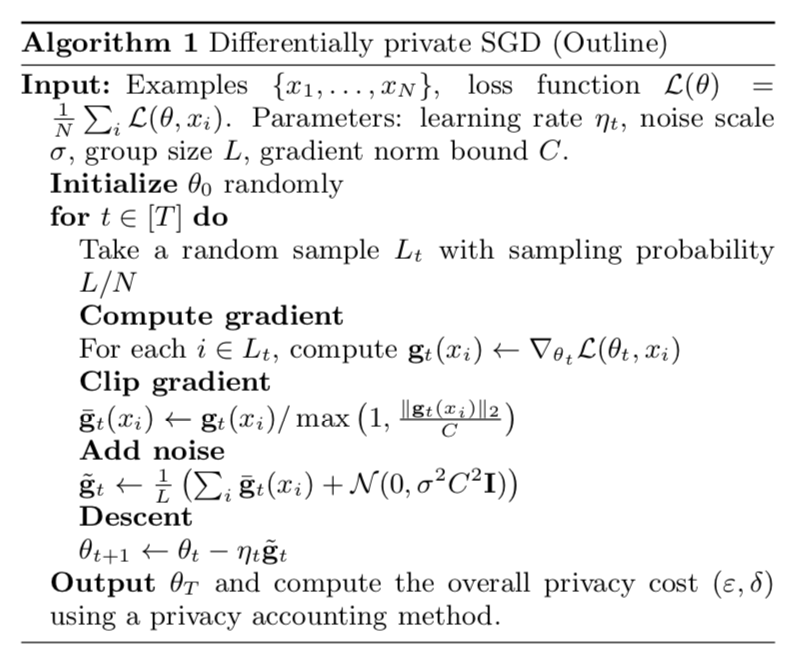
\includegraphics[width=0.8\textwidth]{../images/dpsgd.png}
	\caption{Differentially private SGD}
	\label{}
\end{figure}

\paragraph{Norm clipping} 由于并没有关于梯度大小的先验界限,因此算法中使用$L_2$范数进行修剪。在算法中,如果$\left \| g \right \|_2 \leq C$,则g将被保护,如果$\left \| g \right \|_2 > C$ 则g将会被范数C缩放。
\paragraph{Lots} 在训练时,一个数据集一般被分为不交叉的多个batch,而此处的lot则指的是每次从整个数据集中随机取L条数据,每条数据被取出的概率是$q=L/N$,类似于,batch是不放回抽样,lot是放回抽样。
\paragraph{Privacy accounting} 差分隐私SGD需要计算总体隐私成本,可利用隐私的组合性质逐个进行计算,最后再求和。
\paragraph{Moments accountant} 


\section{The algorithmic foundations of differential privacy\cite{dwork2014algorithmic}}
\subsection{Basic Terms}
\subsubsection{Formalizing differential privacy}

\paragraph{概率单纯形(Probability Simplex)} 离散集合B上的概率单纯形定义为:
\begin{equation}
	\Delta (B) = \left \{ x \in R^{|B|}: x_i \geq \mbox{0 for all i and } \sum_{i=1}^{|B|} x_i=1 \right \}
\end{equation}
它是一个向量集合,其元素是一个概率表,一个|B|维向量,此向量每个元素代表一个概率,所有元素之和为1。
\paragraph{随机算法(Randomized Algorithm)} 定义域为A,值域为B的概率算法与一个映射$M:A \rightarrow \Delta (B)$相关联,对算法的输入$a \in A $,其输入为 $b \in B$,b的值是一个随机变量,满足分布$M(a)$。
\paragraph{数据库距离} 假设数据库中的记录都来自于集合$\chi$,$x_i$的值为自然数,表示集合$\chi$中的第i个元素出现在数据库x中的次数。这样就可以用$x\in \mathbb{N}^{|\chi |}$来表示数据库。 两个数据库之间的距离定义为为其$l_1$范数,即:$\left \| x-y \right \|_1$。
\paragraph{隐私损失(Privacy loss)} 观察$\xi$引起的隐私损失定义为:
\begin{equation}
	L^{(\xi)}_{M(x)||X(y)}=ln(\frac{Pr[M(x)=\xi]}{Pr[M(y)=\xi]} )
\end{equation}
此值若为正,则说明一个观察结果更可以由x引起,若为负,则说明结果更可能由y引起。($\epsilon, \delta$)-差分隐私可以确保,对于所有的邻接集合x,y,隐私损失的绝对值都至少以概率$1-\delta$被限制在$\epsilon$ 以内。
\paragraph{后处理(Post-processing)} 差分隐私对后处理是免疫的,也就是说,如果一个算法保护了隐私,那对这个算法的结果做任何处理都不会增加隐私损失。
\subsection{Basic Techniques and Composition Theorems}
\subsubsection{The laplace mechanism}
\paragraph{$l_1$-敏感度} 函数f的$l_1$-敏感度是:
\begin{equation}
	\Delta f = \max_{x, \in \mathbb{N}^{|\chi|} \atop \left \| x-y \right \|_1=1} \left \| f(x)-f(y) \right \|_1
\end{equation}
$l_1$-敏感度是决定响应查询有多精确的一个重要参数。$l_1$-敏感度给出了一个上界:为了保护隐私我们必须在多大程度上干扰输出。为了达到这个目的,我们很自然想到用一个噪声随机变量来实现差分隐私。
\paragraph{Laplace分布} 以0为中心,尺度为b的Laplace分布的概率密度函数定义为:
\begin{equation}
	Lap(x|b)=\frac{1}{2b	}\exp(-\frac{|x|}{b}).
\end{equation}

\paragraph{Laplace机制} 对于函数$f:\mathbb{N}^{|\chi|} \rightarrow \mathbb{R}^k$,$M_L$是满足$\epsilon$-差分隐私的输出结果,$Y_i$是独立同分布的随机变量,且$Y_i \sim Lap(\Delta f / \epsilon$,有:
\begin{equation}
	M_L(x, f(\cdot), \epsilon )=f(x) + (Y_1, ... , Y_k)
\end{equation}
Laplace机制捕获f的输出,并简单地加上尺度为$\Delta f / \epsilon$的Laplace随机变量进行干扰,使得输出满足$\epsilon$-差分隐私。
\paragraph{示例3.1 计数查询} 计数查询被描述为:数据集中满足条件P的元素有多少个。其敏感度为$\Delta f = 1$,因此可以通过添加满足$Lap(1/\epsilon)$的噪声使其满足$\epsilon$-差分隐私。如果是由任意但固定的m个计数查询组成的联合查询,可表示为$f_m:\mathbb{N}^{|\chi|} \rightarrow \mathbb{R}^m$,由于改变一条数据就有可能改变所有的输出,因此其敏感度为$\Delta f_m = m$,因此可以通过添加满足$Lap(m/\epsilon)$的噪声使其满足$\epsilon$-差分隐私。
\paragraph{示例3.2 直方图查询} 直方图查询描述的是:如果将数据集中的所有元素进行不交叉分类,每个类别中各有多少元素。其敏感度为$\Delta f = 1$。
\paragraph{定理 3.8} 令 $f_m:\mathbb{N}^{|\chi|} \rightarrow \mathbb{R}^k$,$y=M_L(x, f(\cdot), \epsilon )$,则:
\begin{equation}
	Pr[\left \| f(x)-y \right \|_\infty \geq \ln(\frac{k}{\delta})\cdot (\frac{\Delta f}{\epsilon})] \leq \delta
\end{equation}
$\left \| f(x)-y \right \|_\infty$ 表示任意大小的数据集,因加入干扰导致错误的数据条数。此定理可用于计算在满足指定差分隐私的情况下,在一个置信区间内出现错误的数据条数的上界。
\paragraph{示例 3.3 姓氏统计} 假设我们要统计一个数据集中所有人的姓氏分别是多少个,候选姓氏总数一共有10000个,可以表示为:$f:\mathbb{N}^{|\chi|} \rightarrow \mathbb{R}^10000$。这是一个直方图查询,因此$\Delta f=1$。假设我们希望查询满足(1,0)-差分隐私,置信度为95\%,由于$\ln(10000/0.05) \approx 12$,则有:$Pr[\left \| f(x)-y \right \|_\infty \geq 12] \leq 0.05$,也就是说,在满足(1,0)-差分隐私,置信度为95\%的情况下,数据因干扰出错的数量上界为12条。由于定理本身对数据集大小没有规定,因此如果我们使用的是一个数量为3亿的国家人口数据集,这将是一个非常低的错误率。
\paragraph{Report Noisy Max} 考虑查找m元计数查询的最大值的问题:m元计数查询中每一个计数结果都加上噪声$Lap(1/\epsilon)$,返回其中最大的那个值。此算法满足($\epsilon$,0)-差分隐私。
\subsubsection{指数机制}
\paragraph{指数机制} 用于这样的场合:需要返回一个最大值,但不能给值直接加上noise,因为这会导致返回错误的值(非最大值加上噪声后可能会变成最大值)。例如,返回拍卖中的最佳出价,但要求不泄露最终价格。指数机制基于效用函数$u: \mathbb{N}^{|\chi|} \times R \rightarrow \mathbb{R}$来定义,R是离散的输出结果。
\subsubsection{组合定理}
\paragraph{定理 3.14} 有$M_1: \mathbb{N}^{|\chi|} \rightarrow R_1$,$M_2: \mathbb{N}^{|\chi|} \rightarrow R_2$分别满足$\epsilon_1, \epsilon_2$-差分隐私,则他们的组合$M_{1,2}(x)=(M_1(x),M_2(x))$满足$\epsilon_1+\epsilon_2$-差分隐私。
\paragraph{支撑集} 随机变量X的支撑集表示为Supp(X),一个概率的支撑集就是所有概率密度非零部分的集合。
\paragraph{KL-散度} 定义为:
\begin{equation}
	D(Y \parallel Z) = \mathbb{E}_{y\sim Y}\begin{bmatrix} \ln \frac{Pr[Y = y]}{Pr[Z = y]} \end{bmatrix}
\end{equation}
表示两个随机变量之间的“距离”,但是它不是对称的,也不满足三角不等式,当Supp(Z)不包含Supp(Y)的时候甚至有可能是无穷大。
\paragraph{Max 散度} 定义为:
\begin{equation}
	D_{\infty}(Y \parallel Z) = \max_{S\subseteq Supp(Y)} \begin{bmatrix} \ln \frac{Pr[Y \in S]}{Pr[Z \in S]} \end{bmatrix}
\end{equation}
\paragraph{$\delta$-近似Max散度} 定义为:
\begin{equation}
	D_{\infty}^{\delta}(Y \parallel Z) = \max_{S\subseteq Supp(Y):Pr[Y \in S]\geq \delta} \begin{bmatrix} \ln \frac{Pr[Y \in S] - \delta}{Pr[Z \in S]} \end{bmatrix}
\end{equation}
\paragraph{备注 3.1} 机制M是$\epsilon$-差分隐私的,当且仅当,对两个邻接数据集x,y有:
\begin{enumerate}
	\item $D_{\infty}(M(x) \parallel M(y)) \leq \epsilon$ and $D_{\infty}(M(y) \parallel M(x)) \leq \epsilon$
	\item $D_{\infty}^{\delta}(M(x) \parallel M(y)) \leq \epsilon$ and $D_{\infty}^{\delta}(M(y) \parallel M(x)) \leq \epsilon$
\end{enumerate}
\paragraph{统计距离(statistical distance)} 两个随机变量之间的统计距离定义为:
\begin{equation}
	\Delta(Y,Z) \overset{\underset{\mathrm{def}}{}}{=} \max_S(Pr[Y \in S]-Pr[Z \in S])
\end{equation}
如果有$\Delta(Y,Z) \leq \delta $,我们称Y和Z是$\delta$-近邻(close)。
\paragraph{引理 3.17}
\begin{enumerate}
	\item $D_{\infty}^{\delta}(Y \parallel Z) \leq \epsilon \Leftrightarrow \exists Y': \Delta(Y,Y')\leq \delta \wedge D_{\infty}(Y' \parallel Z)\leq \epsilon$
	\item $D_{\infty}(Y \parallel Z)\leq \epsilon \wedge D_{\infty}(Z \parallel Y)\leq \epsilon \Leftrightarrow \exists Y',Z': \Delta(Y,Y')\leq \delta/(e^\epsilon+1) \wedge \Delta(Z,Z')\leq \delta/(e^\epsilon+1) \wedge D_{\infty}(Y' \parallel Z') \leq \epsilon$
\end{enumerate}
\paragraph{引理 3.18} $D_{\infty}(Y \parallel Z) \wedge D_{\infty}(Y \parallel Z) \Rightarrow D(Y \parallel Z)\leq \epsilon \cdot (e^\epsilon-1 )$
\paragraph{高级组合的使用场景} 我们的定义要考虑以下两个场景:
\begin{itemize}
	\item 对同一个数据集重复使用同样的差分隐私算法;
	\item 针对使用了同一个个体数据的不同数据集,重复利用同样的差分隐私算法。
\end{itemize}
我们考虑两个实验:
\begin{itemize}
	\item 两个实验使用同一组预定义的隐私机制F;
	\item 实验由攻击者A进行,每个实验对数据集进行k次操作(k重);
	\item A每次使用机制$M_i$和参数$w_i$进行操作,针对两个实验输入两个邻接数据集$x_i^0$和$x_i^1$,并接收到结果$y_i \in_R M_i(w_i,x_{i,b})$(针对实验b)。
	\item $V_b$表示实验b获得的结果$(y_1,...,y_k)$;
	\item A在实验过程中是有记忆的(stateful),他可以根据情况自由选择数据集、机制和参数;
	\item A总是认为数据集$x_i^0$包含Bob的信息,而$x_i^1$没有;
	\item 我们要求的隐私保障是:攻击者不能分辨数据集中是否包含Bob的信息。
\end{itemize}
\paragraph{k重自由组合下的$\epsilon$-差分隐私} 如果一组机制F有$D_{\infty}(V^0\parallel V^1)\leq\epsilon$,我们就称F满足k重自由组合下(under k-fold adaptive composition)的$\epsilon$-差分隐私。
\paragraph{定理3.20 高级组合} 一组$(\epsilon, \delta)$-差分机制的k重自由组合满足$({\epsilon}', k\delta+{\delta}')$-差分隐私,其中: ${\epsilon}'=\sqrt{2k\ln(1/{\delta}'\epsilon)} + k\epsilon(e^\epsilon-1)$.
\paragraph{Laplace vs. Gauss} 我们可以使用Gauss噪声代替Laplace噪声,此时,我们需要使用$l_2$敏感度:
\subparagraph{$l_2$-敏感度} 函数$f: \mathbb{N}^{|\chi|} \rightarrow \mathbb{R}^k$的$l_2$-敏感度定义为:
\begin{equation}
	\Delta_2(f)=\max_{x,y \in \mathbb{N}^{|\chi|} \atop \left \| x-y \right \|_1=1} \left \| f(x)-f(y) \right \|_2
\end{equation}
\subparagraph{定理3.22} 对于$c^2 > 2\ln(1.25/\delta)$,满足参数$\sigma \geq c\Delta_2(f)/\epsilon$的Gauss机制满足$(\epsilon, \delta)$-差分隐私。





\section{Not Just Privacy: Improving Performance of Private Deep Learning in Mobile Cloud\cite{arden}}
\subsection{Introduction}
\paragraph{} 为了实现移动端的深度学习,一般有两种做法:1. 减小DNN的规模;2. 将大型DNN划分到各个设备和云端进行。前者会导致性能下降和无法控制的能量消耗;后者通过将DNN的前几层设置在移动设备上,而后几层部署在云端来实现。为了平衡效用和隐私,通常客户端会把用户数据进行转换再上传到云端,然而,即便传输的不是原始数据也会产生隐私泄露。
\paragraph{ARDEN} 将网络分割为移动端和云端两个部分,DNN的浅层被部署在移动端,用于将原始数据转换成低级特征。

\subsection{The Proposed Framework}
\subsubsection{Overview}
\paragraph{} ARDEN 将DNN划分为移动端和云端,浅层部署在移动端,它的参数是固定的,其参数值可以通过迁移学习而来;云端的参数则通过训练进行调参。
\paragraph{推理阶段} 敏感数据首先被移动端的浅层进行转换处理,为保证隐私,数据还同时被进行nullification和随机噪声处理,之后才被传输到云端进行深层推理。
\paragraph{训练阶段} 使用与敏感数据相同类型的公开数据进行训练,同时,提出了一个噪声训练方法,将原始数据与生产数据同时用于训练。
\subsubsection{Differentially private transformation}
\paragraph{} 为了保护隐私,需要在本地将数据进行干扰。直观的方法是在结果中直接加入Lap噪声,但由于获取总体敏感度比较困难,因此这会导致加入过的噪声而使效用减低。另外,这种方法也无法提供高度定制化的隐私要求,例如隐去某个高度敏感的字段。因此,本文提出了包括nullification和layer-wise扰动两种机制。

\newpage
\section{Learning privacy preserving encodings through adversarial training\cite{pittaluga2019learning}}
\subsection{Introduction}
\paragraph{} 图像、视频等高纬度数据在分享过程中总是会不经意地泄露一些信息。本文试图找到一种方法,即可以保证信息的有效共享,又能防止隐私泄露。
\paragraph{} 本文利用对抗训练去学习一种编码,以阻止分类器通过编码过的数据去成功地推导隐私信息。文章演示了在场景识别的应用中,在提升正样本识别率的同时如何降低负样本的识别率。在作为baseline的模糊操作都不能阻止场景识别的情况下,本文提出的编码器可以成功地降低负样本场景识别率。
\subsection{Learning Privcate Encoding Functions}
\paragraph{} 本文框架基于这样的前提:1. 用于训练编码器的训练集打上了隐私属性值的标签,一旦编码器训练完成,我们将试图对敏感值估计器的训练能力进行限制。2. 当编码器训练完成后,攻击者能够利用编码后的带标签的数据训练估计器,我们需要对这样的估计器的性能进行限制。
\subsubsection{Privacy as Adversarial Objective}
\paragraph{}对整个框架进行形式化定义:
	\subparagraph{编码器} $E: \mathbb{R}^N \rightarrow \mathbb{R}^{N'}$,输入样本$x \in \mathbb{R}^N$,$E(x)_i$表示E(x)的第i个元素。
	\subparagraph{隐私属性} $u(x) \in \mathbb{U}$。编码器的目标就是要保护隐私属性的值$u(x)$免于纰漏。
	\subparagraph{参数化的估计器} $\hat u = \Phi(x';\theta_u)$
	\subparagraph{估计器的损失函数} $L(\hat u, u): \mathbb{U} \times \mathbb{U} \rightarrow R$,L越小,则估计出的敏感值越准确。
	\subparagraph{估计器的训练目标} $I(E;u) = \underset{\theta_u}{\min}\underset{p(x)}{\mathbb{E}}\,L(\Phi(E(x);\theta_u),u(x))$. 调整$\theta_u$,使得估计器的平均损失最小。  
	\subparagraph{编码器的训练目标} $E = \arg\max_E I(E;u)$. 使得I最大的那个E。
	\paragraph{避免模型坍塌} 从训练目标可以看出,这将引发模型坍塌问题,致使最终E(x)变为常数。为避免这个问题,本文对编码器的输出做了一个限制:要求$\mathbb{E}E(x)_i = 0, \mathbb{E}E(x_i^2) = 1$,即均值为0,方差为1.
	\paragraph{保护特定的属性} 编码器$E = \arg\max_E I(E;u)-\alpha I_v(E)$可以在编码的同时保护特定的属性v。即要求I(E;u)尽可能大的同时,I(E;v)尽可能小。
\subsubsection{Architecture and Optimization}

\subsection{Experimental Results}
\paragraph{基础}
\subparagraph{数据集} Places-365。本文从数据集中取两个组,每个组10个类别,用于构造“平衡”样本数据集。数据集的正样本就是其中一个类别,而负样本则从同一个组中的其余9个类别中随机抽取。
\subparagraph{实验任务} 进行一次二分类:一个图片是否属于某个指定的分类。训练后的模型应当可以抑制某个特定类别(降低特定类别的分类精度),同时也要评估编码器对另外的类别的分类精度的影响。

\paragraph{编码器训练} 本文训练4个编码器,用于抑制4种类别的分类,分别是:arch, army base, airport terminal, airfield。另外还训练了第五个编码器,用于抑制“army base”,同时避免对“airport terminal”的识别造成影响,此时取$\alpha=1/4$。
\paragraph{评估}
\subparagraph{基线} 对图像进行模糊后得到的分类结果。
\subparagraph{} 分别训练两个编码器:army base 和 airport terminal,同时训练一个抑制army base但提升airport terminal的编码器。
\subparagraph{} 图3的第1列展示了图像经过了编码器后,输入分类器得到的训练精度和验证精度,表明编码器可以成功地降低分类精度(进行抑制);第2、3列分别演示了不同编码器对army base和airport terminal分类器的影响,输入分类器的图像是经过了编码器得到的输出结果。可以看成,当编码器固定后,即便使用经过编码的图像对分类器进行训练,分类器依然不能得到很好的精度。

\section{Gp-gan: Gender preserving gan for synthesizing faces from landmarks\cite{gpgan2018}}
\subsection{Introduction}
\paragraph{动机} 面部landmark有一系列优点,本文研究怎么将landmark用于高级别(high-level)的面部分析任务上。目前只需要68个面部landmark就可以完成性别预测,本文将通过landmark生成面部图像,以此来提升性别预测的性能。
\paragraph{贡献} 1. 在保护性别隐私情况下,第一次使用landmark生成面部图像;2. 提出了基于GAN的框架;

\subsection{Proposed Method}
\paragraph{生成器} 使用U-Net和DenseNet
\paragraph{判别器} 使用PatchGAN
\paragraph{目标函数} $L=L_A+\lambda_PL_P+\lambda_CL_C+\lambda_1L_1$
\subparagraph{对抗损失} 定义为一组生成图片的熵:
\begin{equation}
	L_A=-\frac{1}{N}\sum_{i=1}^N\log(D(\hat x_i))
\end{equation}
\subparagraph{Perceptual loss} 定义为:$L_P=\left \| V(\hat x)-V(x) \right \|_1$
\subparagraph{Gender preserving loss} 描述生成的图像与真实图像之间的性别误差,定义为:
\begin{equation}
	L_C=-\frac{1}{N}\sum_i(C(x_i)\log(C(\hat x_i)) +(1-C(x_i))\log(C(\hat x_i)))
\end{equation}
C表示预定义好的性别分类网络,本文使用VGG-16.
\subparagraph{L1 loss} 描述生成的图像与真实图像之间的重建误差,定义为:
\begin{equation}
	L_1= \left \| G(\hat x)-x \right \|_1
\end{equation}
\subsection{Experiments}
\paragraph{} 实验发现,使用GPGAN由landmark生成的图像可以很好地保存性别属性,生成图像的性别正确率超过90\%.

\section{Deepfool: a simple and accurate method to fool deep neural networks\cite{deepfool}}
\subsection{Introduction}
\paragraph{} Deepfool的目的是找出使分类器做出错误判断的最小扰动。
\subsection{DeepFool for binary classifiers}
\paragraph{} 二分类器通过一个超平面将所有样本点分开,为了实现扰动,需要使样本点偏移到超平面的另外一边。具体的定义为:
\subparagraph{$\hat k$在点x处的鲁棒性} 调整向量r,使得f(x)的符号改变,且r距离原点最近:
\begin{equation}
	\Delta(x;\hat k) := \min_r \left \| r \right \|_2 \mbox{ subject to } \hat k(x+r)\neq \hat k(x).
\end{equation}
\subparagraph{分类器$\hat k$的鲁棒性} 扰动r到原点距离与x到原点的距离之比的均值:
\begin{equation}
	\rho_{adv}(\hat k) = \mathbb{E}_x\frac{\Delta(x;\hat k)}{\left \| x \right \|_2}
\end{equation}
\subparagraph{划分超平面} 定义为:$\mathfrak{F}: {x:f(x)=0}$.
\subparagraph{点到超平面的距离\cite{2016机器学习}} 定义为:
\begin{equation}
	r = \frac{|w_Tx+b|}{\left \| w \right \|}
\end{equation}

\section{Protecting visual secrets using adversarial nets\cite{raval2017protecting}}
\subsection{Introduction}
\paragraph{} 当我们一直在追求神经网络效率的同时,也要注意对所捕获的图像中隐私内容的保护。本文采用一种对抗扰动机制来隐藏图像中的隐私内容。

\subsection{Adversarial Perturbation Mechanism}
\paragraph{} 框架有两个网络组成:攻击者网络A和混淆器网络O。框架描述:
	\subparagraph{} X: 所有图像的集合, $X_S \subseteq X$: 带有敏感数据的图片集合,$X_U = X \\ X_S$:公开图片。
	\subparagraph{混淆器O} $O(x, \theta_O) \in X$表示混淆结果,其符合公开图片的分布。
	\subparagraph{攻击者网络A} $A(x, \theta_A)$表示攻击者对于图片x含有隐私信息的概率。
	\subparagraph{攻击者网络A的优化条件} 找到$\theta_A$,使得当x含有敏感数据时A最大,A是公开图片是A最小。
		\begin{equation}
			\begin{split}
				\arg\max_{\theta_A}\mathbb{E}_{x\in X_S}A(x,\theta_A) &+ \mathbb{E}_{x\in X_U}(1-A(x,\theta_A)) \\
					& +\mathbb{E}_{x\in X_S}A(O(x, \theta_O),\theta_A) \\
					& +\mathbb{E}_{x\in X_U}(1-A(O(x, \theta_O),\theta_A))
			\end{split}
		\end{equation}
	\subparagraph{混淆器O的优化条件} 找到$\theta_O$,使得任意图片对攻击者网络A的输出及效用损失(utility loss, $L_U$)最小。
		\begin{equation}
			\begin{split}
				\arg\min_{\theta_O}\lambda & \mathbb{E}_{x \in X} A(O(x, \theta_O),\theta_A) \\
					& +(1-\lambda)\mathbb{E}_{x\in X}L_U(x, O(x,\theta_O))
			\end{split}
		\end{equation}
	$\lambda$可用于权衡隐私和效用,本文中效用损失定义为$L_1$范数:$L_U(x,y)=\left \| x -y \right \|_1$.

\subsection{实验}
\paragraph{数据集} CIFAR10,选择其中两个分类:horse和airplane。一共有10000个训练样本和2000个测试样本,组成了公开图片$X_U$,利用这些图片,本文在每张图片上生成一个随机的二维码当做是敏感信息,从而生成$X_S$。


\section{Towards Deep Learning Models Resistant to Adversarial Attacks}
\subsection{Introduction}
\paragraph{动机} 已有不少研究可对抗基于深度学习的分类器,抵御对抗选择输入攻击已经成为深度学习网络设计的一个重要目标。本文研究如何提供一个系统针对对抗输入的健壮性。
\paragraph{存在的问题} 目前提高健壮性的方法包括detection distillation, feature squeezing和对抗样本检测等。然而,这些方法并不能对他们所提供的保障给出一个好的理解,无法保证攻击无法找到对抗性样本。
\paragraph{研究内容} 本文在健壮性优化的角度下,研究神经网络的对抗健壮性。
\subsection{对抗健壮性的优化视图}


\newpage
\section{Censoring Representations with an Adversary\cite{censoring}}
\paragraph{} 本文要解决的问题是:我们希望提供数据给第三方,但确保第三方无法计算得到关键的敏感数据。相关的应用主要有两类:公平分类和图像匿名化。
	\subparagraph{公平分类} 一个分类决策是无歧视的,不依赖于敏感字段。
	\subparagraph{图像匿名化} 在传输图像给第三方前,移除图片中的一些敏感信息。本文所使用的方法在训练模型时无需使用对齐的样本,仅需要两组分类好的样本即可。
\paragraph{公平和歧视的形式化定义} 考虑一个分类任务,输入空间是$X \subset \mathbb{R}^n$,输出为标签集$Y = \{0,1\}$和隐私$S=\{0,1\}$。分类器定义为:$\eta : X \rightarrow Y$。
	\subparagraph{公平} 定义为:$P(\eta(X)=1|S=1))=P(\eta(X)=1|S=0)$,也就是说,无论敏感数据是什么样的,分类为同一个标签的概率都是一样的。
	\subparagraph{歧视}定义为:
\paragraph{审查表示} 的目的是学习一种表示$R=Enc(X)$,使得它能够保留X用于预测Y的那部分信息,但对于敏感数据S是独立的。损失函数可以表示为:$L=\alpha C(X,R) + \beta D(S,R) + \gamma E(Y,R)$,他包括三个部分:
	\subparagraph{C} 是从R重构X的成本;
	\subparagraph{D} 是R和S之间依赖性的度量。
	\subparagraph{E} 是由R预测Y的误差。

\newpage
\section{The Secret Sharer: Measuring Unintended Neural Network Memorization \& Extracting Secrets\cite{secretsharer}}
\paragraph{} 机器学习模型可能会在无意中泄露秘密(例如“自动完成文本”功能),因此,即便这种情况很少见,一个好的模型也应当假设它的存在。在机器学习过程中,无意的记忆很难避免,只有在训练过程中使用差分隐私技术才能消除隐私纰漏问题。
\paragraph{} 本文假设存在一个威胁模型:一些用户通过输入大量不同的数据试探模型。

\newpage
\section{Poster: Image Disguising for Privacy-preserving Deep Learning\cite{imagedisguising}}

\paragraph{动机} 深度学习经常使用外部资源(GPU等),这可能会导致隐私泄露。由于深度学习本身很强大,因此即便是经过伪装的图片它也能够分辨。因此,本文要讨论的问题就是怎么设计比较合理的机制,使得原始图片可以很好地被伪装(在视觉上和算法上均不能重构),同时又能保留深度学习需要的特征。
\paragraph{图像伪装} 假设有一个图片集${(X_i,y_i}$,伪装机制$T_K$将其转换成${(T_K(X_i),y_i}$,$D_T$是一个以$T_K(X_i)$作为输入的深度网络,其输出为$\hat y = D_T(T_K(X))$。
	\subparagraph{Block-wise Permutation} 将图像分割成小块,并打乱后重拼。然而,这样的机制对于隐藏图片内容毫无意义,因为根据小块的边缘文理之间的关系可以很容易地恢复原始图像。
	\subparagraph{Randomized Multidimensional Transformations} 对图像X做一个转换:$XR+\Delta$,其中$\Delta$是一个随机噪声。


\newpage
\section{Vgan-based image representation learning for privacy-preserving facial expression recognition\cite{pprl-vgan}}
\paragraph{}自动面部表情识别是人机交互的重要组件,目前大量表情识别系统依赖于高清图片,忽略了用户的视觉隐私。目前很多方法,为了保护隐私对图像进行像素化或模糊,这降低了效用。
\paragraph{} 本文利用VGAN将图片转换成可用于表情识别的表示,以及表情相同但指定id的图像。
\begin{figure}[H]
	\centering
	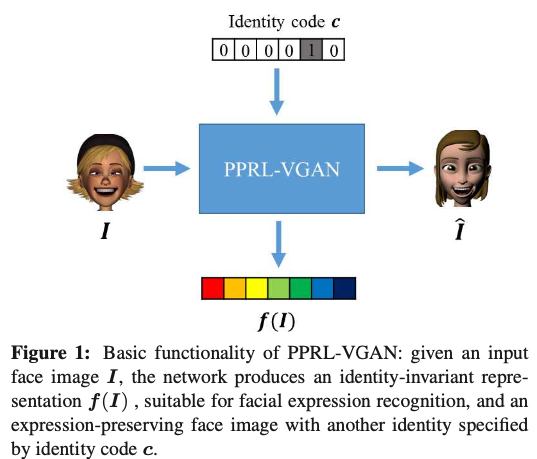
\includegraphics[width=0.6\textwidth]{../images/pprl-vgan.png}
	\caption{}
	\label{laplace-distribution}
\end{figure}

\paragraph{} PPRL-VGAN的网络如下图:
\begin{figure}[H]
	\centering
	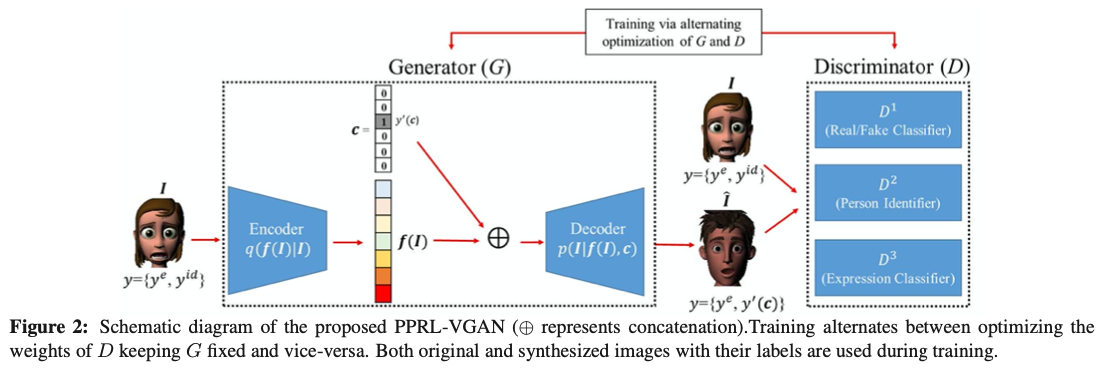
\includegraphics[width=1.0\textwidth]{../images/pprl-vgan-network.png}
	\caption{}
	\label{laplace-distribution}
\end{figure}
\paragraph{} 给定一个图像I,用户标签为$y^{id}$,表情标签为$y^e$。模型的主要目的是
\begin{enumerate}
	\item 学习一个身份不变的面部图像表示f(I),用于面部表情识别;
	\item 合成一个具有相同表情,并具有指定面容的图像$\hat I$。
\end{enumerate}

\paragraph{判别器} 模型有三个判别器
	\subparagraph{} $D^1$ 用于判断图像是真实图像还是合成图像;
	\subparagraph{} $D^2$ 用于判断用户身份是否在输入集合中;
	\subparagraph{} $D^3$ 用于对表情进行分类。

\newpage
\section{Learning to Anonymize Faces for Privacy Preserving Action Detection\cite{anonymize-faces}}
\paragraph{} 本文开发一个视频人脸匿名器。在智能家庭应用中,智能摄像头可能需要通过读取用户动作来进行判断,但此类判断并不需要用户隐私信息(比如脸部信息)。本文开发的匿名器就是将视频中的人脸信息进行一个匿名化。
\begin{figure}[H]
	\centering
	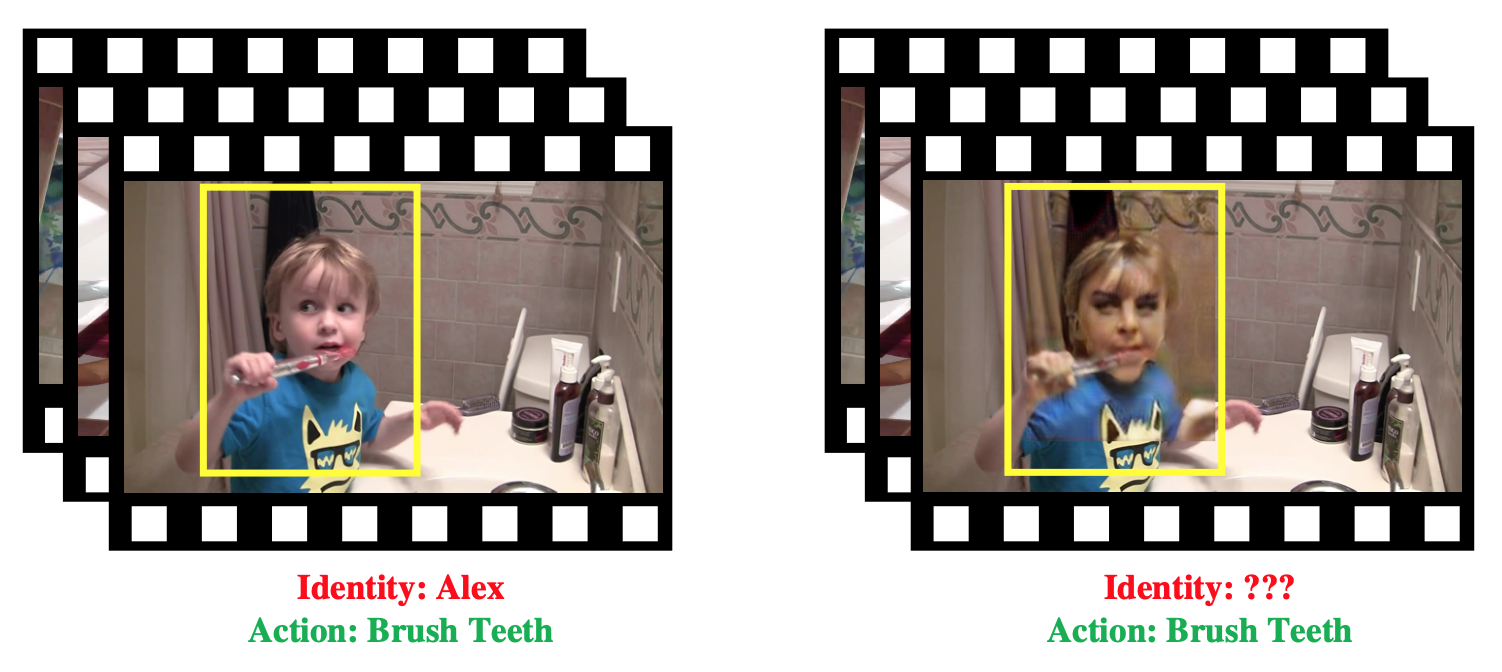
\includegraphics[width=0.9\textwidth]{../images/face-anonymity.png}
	\caption{}
	\label{laplace-distribution}
\end{figure}
\paragraph{} 本文的目标是在匿名化视频中的人物的同时还能够识别动作。总体框架如图:
\begin{figure}[H]
	\centering
	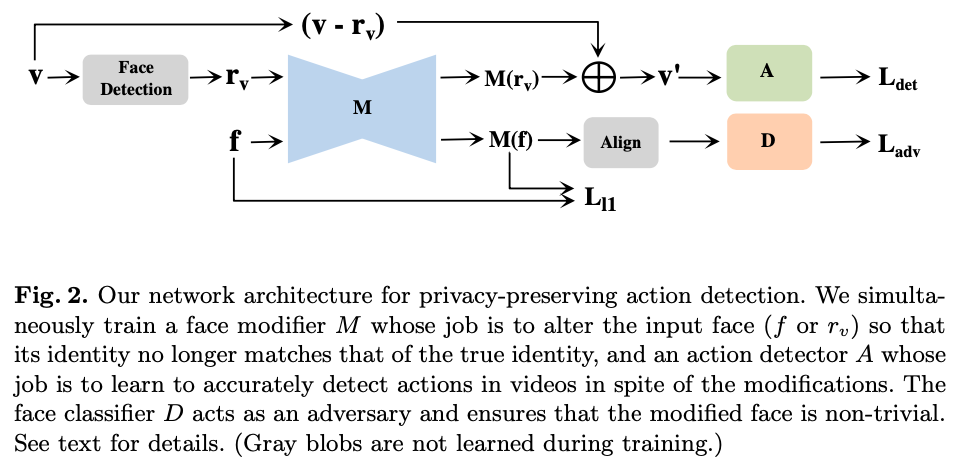
\includegraphics[width=0.9\textwidth]{../images/face-anonymity-framework.png}
	\caption{}
	\label{laplace-distribution}
\end{figure}
\paragraph{} 需要学习3个主要组件:
	\subparagraph{编码器M} 用于将输入的图像匿名化;
	\subparagraph{动作识别器A} 用于识别视频中人的动作;
	 \subparagraph{面部分类器D} 用于对图像中的人进行面部识别。


\newpage
\section{Efficient Decision-based Black-box Adversarial Attacks on Face Recognition\cite{blace-box-attack-fr}}



\newpage
\bibliographystyle{ieeepes}
\bibliography{../Saliency}
\end{document}